\documentclass{article}

\usepackage{tikz}
\usetikzlibrary{arrows.meta}

\begin{document}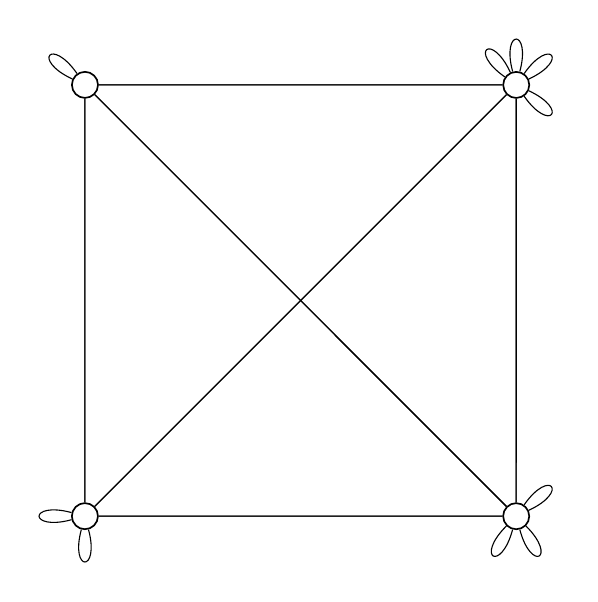
\begin{tikzpicture}[>={Latex},
  default/.style={draw=black, semithick, solid, fill=white, solid},
  every loop/.style={looseness=16}]
\node[default, circle] (A) at (-2.73838, 2.738863) {};
\node[default, circle] (B) at (-2.738845, -2.738363) {};
\node[default, circle] (C) at (2.738375, -2.738863) {};
\node[default, circle] (D) at (2.73885, 2.738363) {};
\draw [] (A) -- (B) ;
\draw [] (A) -- (C) ;
\draw [] (A) -- (D) ;
\path (A) edge [in=125,out=155,loop]  (A);
\draw [] (B) -- (A) ;
\draw [] (B) -- (C) ;
\draw [] (B) -- (D) ;
\path (B) edge [loop left]  (B);
\path (B) edge [loop below]  (B);
\draw [] (C) -- (A) ;
\draw [] (C) -- (B) ;
\draw [] (C) -- (D) ;
\path (C) edge [in=225,out=255,loop]  (C);
\path (C) edge [in=285,out=315,loop]  (C);
\path (C) edge [in=25,out=55,loop]  (C);
\draw [] (D) -- (A) ;
\draw [] (D) -- (B) ;
\draw [] (D) -- (C) ;
\path (D) edge [in=25,out=55,loop]  (D);
\path (D) edge [loop above]  (D);
\path (D) edge [in=115,out=145,loop]  (D);
\path (D) edge [in=305,out=335,loop]  (D);
\end{tikzpicture}
\end{document}
